\documentclass[12pt, a4paper]{article}
% Packages
\usepackage[english]{babel}
\usepackage[letterpaper,top=2cm,bottom=2cm,left=3cm,right=3cm,marginparwidth=1.75cm]{geometry}
\usepackage[colorlinks=true, allcolors=blue]{hyperref}
\usepackage{parskip}
\usepackage{graphicx}

\graphicspath{{./photos/}}

\title{Predicting Customer Turnover}
\author{Govind Tanda}

\begin{document}
\maketitle

% INTRODUCTION 
\section{Introduction}

In the modern world, there is a lot of competition between businesses to offer the best deals in order to persuade customers to do business with them. These plentiful options make it harder for companies to retain customers since another company may offer different deals or services to entice customers to join them, this has made preventing customer churn a necessity for businesses since they need to be able to analyze when a customer is at risk to leave and to know why they're leaving to stop them from becoming part of the churn. Analyzing customer churn allows companies to mitigate possible losses by being able to do risk-analysis on your customer and improving relationships with them before they get to the point of leaving. By doing an analysis on why customers are leaving, the company can recognize parts of their service that need improving to keep customers happy.
 
In the telecommunications business, there can be roughly 2.2\% customer churn monthly, which roughly results in over 25\% of customers churning within a year \cite{10.5555/555454}. These churners can cost telecommunication businesses between \$300 - \$600 to acquire new customers \cite{WEI2002103}. Churn analysis can provide great benefits to companies by saving costs since losing customers can be expensive. A lot of the cost that is incurred because of churn can be related to customer acquisition costs since for each customer that is lost there needs to be someone that can replace them. To create new customers, a company must be willing to invest in customer acquisition which can result in costly marketing campaigns. With the many options available now, it is not uncommon for customers to frequently swap their services to another provider in order to receive better services or prices \cite{WEI2002103}.  This costly acquisition fee and knowing that customers frequently churn can create an incentive for businesses to produce methods that reduce churn since the cost of retaining customers is less costly than acquiring new customers \cite{WEI2002103}.
 
As we can see there is great benefit for companies that wish to hold onto customers since reducing churn can increase a company's profits. Although churn analysis can be useful for dealing with customers it can also churn provide useful analytics outside of just customer churn. Churn analysis methods could be applied to other areas where churn can occur such as with employees or students. Churn analysis can help find patterns in customers, students, and employees to create groupings. These groupings can allow companies to find out when a customer is at risk to leave \cite{churn_analysis}. This is useful to companies since they can develop strategies aimed at various groupings and decide the most optimal to minimize customer churning \cite{churn_analysis}. In order to do meaningful customer churn analysis for our telecommunication data, it is important to have relevant data, such as demographics, customer call lengths, billing information, types of subscribed services etc.. \cite{churn1}. In this paper, I am are going to look into using various features provided by a customer data set that provides information about customer data related to telecommunications, ranging from services, charges, tenure and various demographic info about the customer to predict when a customer is at risk to churn and to find the underlying patterns between customers that lead to churning.

This paper will be organized in the following way, Section 2 contains the literature review which expands on sub-topics of customer churn, such as why churn prevention is important, types of churners and which methodologies are being used to predict customer churn. Section 3 contains the methodology, explaining the dataset, feature engineering/modeling building process and model evaluation. Section 4 contains results and discussion. Section 5 contains the conclusion.


\section{Literature Review}
Churn reduction has become an important factor for companies as markets are becoming increasingly competitive. Over 90\% of C-level executives are saying customer churn is their number one concern, but only 43\% have gone as far as investing in reducing churn \cite{ml_techniques_to_predict_churn}. The intense competition puts pressure on companies to develop strong marketing campaigns and to better understand customer needs \cite{customer_retention}. To understand customer needs, many companies have looked towards data mining which has become a common standard in the industry to obtain customer insight since data mining can help find underlying patterns for understanding customers. These underlying patterns can be further used by finding similarities between groups of customers and allow companies to create marketing campaigns directed at specific groups of customers and make decisions for retaining customers based on their grouping \cite{customer_retention}. This raises the question of how can companies get involved to reduce customer churn and reap the benefits of retaining high value customers while also finding the underlying patterns causing customers to churn.\\

 Before looking into methods for churn prediction, we must first understand where churners are coming from and which churners should be targeted for customer retention. The churners are divided into two different groups, the voluntary and non-voluntary \cite{churn_mobile_industry}. The non-voluntary churner is someone who is having their service cancelled by the company, either due to abuse of company policies, a company may have stopped providing services in the area the user's area or the company could have failed thus not having services left to offer \cite{hadden2007computer}. Non-voluntary churners are easier to identify than voluntary churners since usually the company is revoking services from the non-voluntary churners \cite{hadden2007computer}. Voluntary churners on the other hand are revoking their services by their choice. Voluntary churners are likely to leave for fairly common reasons such as bad experiences with customer service, finding better offers with competitors, or simply due to a company offering poor service \cite{customer_loyalty}. It becomes clear that the value for companies is going to come from attempting to retain customers that are starting to fall into the voluntary churners category as they are leaving on their own volition rather than having their services ended by the company.

Many authors have different ideas of what is best when it comes to evaluating churn prediction but what is generally agreed upon is that machine learning will play a large role. The customer churn prediction problem seems to still be an impasse for what is considered to be the optimal model to use, however it seems that most researchers are using multiple algorithms such as logistic regression, decision trees, naive bayes, or artificial neural networks, with some authors suggesting the best practice is to use hybrid-models which can make usage of multiple algorithms to achieve better generalized results \cite{HUANG20121414}, \cite{hybrid_approach}. Mahajan et al, conducted a review of models by various authors and concluded that the best methods to achieve accurate results would come from hybrid methods that made usage of multiple machine learning algorithms rather than singular algorithms \cite{mahajan2017review}. Outside of choosing a method, there is also a need for companies to be continually reviewing their customer data and updating their models so they can keep up with dynamic behaviour of customers \cite{WEI2002103}. No current method is going to be able to provide a one size fits all solution for companies since customer behaviour is also going to vary between geographic location and from company to company. This leads into our question of how can companies make use of methodologies to find potential churners before they become part of the churn?

\section{Methodology}
\subsection{DataSet}
The customer data used for this paper, provides 33 features for 7000 customers that can be used for our predictive model. For the most part, the data seems to be fairly clean, outside of the "churn reason" feature which has 5174 empty or null values. The data set itself was provided initially provided by IBM Cognos Analytics and was uploaded to Kaggle. The data set provides some features that will most likely be used such as:
\begin{itemize}
    \item Tenure with the company
    \item Total charges
    \item Contract type
\end{itemize}

However, the choice of which features will be used will be left up to a feature selection model.

\subsection{Feature Engineering}
To start with feature engineering first I had dropped all of the very correlated data associated with churn value, features such as churn label, churn score, cltv (a customer value score), and churn reason which provided reasons as to why a customer churned were all dropped to avoid a bias and to minimize the number of features in our dataset. Other data that was removed included geographic data such as Country, State, City, zip code and latitude/longitude, since all data was from the California, USA. After dropping these features, ordinal encoding was applied to convert all nominal data to numeric data.

For this project I have decided to use 2 different methods to try and find the optimal features and the optimal number of features to use. The first method was using a simple filter method by checking feature correlation with other features. After the correlation is used, we can look to see if there are any highly correlated features that can be removed to saved processing time when running data through the model but in Figure 1 we can see there is not much correlated data outside of tenure and contract, thus not leaving room for feature reduction.

The second method used was a wrapper method where step forward and step backward feature selection were both used. Step forward feature selection was suggesting similar accuracy as step backward feature selection but was proposing 16 features to be used rather than 10. Both step forward and step backward models were trained using Random Forest Classifier.
\begin{figure}[!ht]
    \centering
    \caption{Feature Correlation Map}
    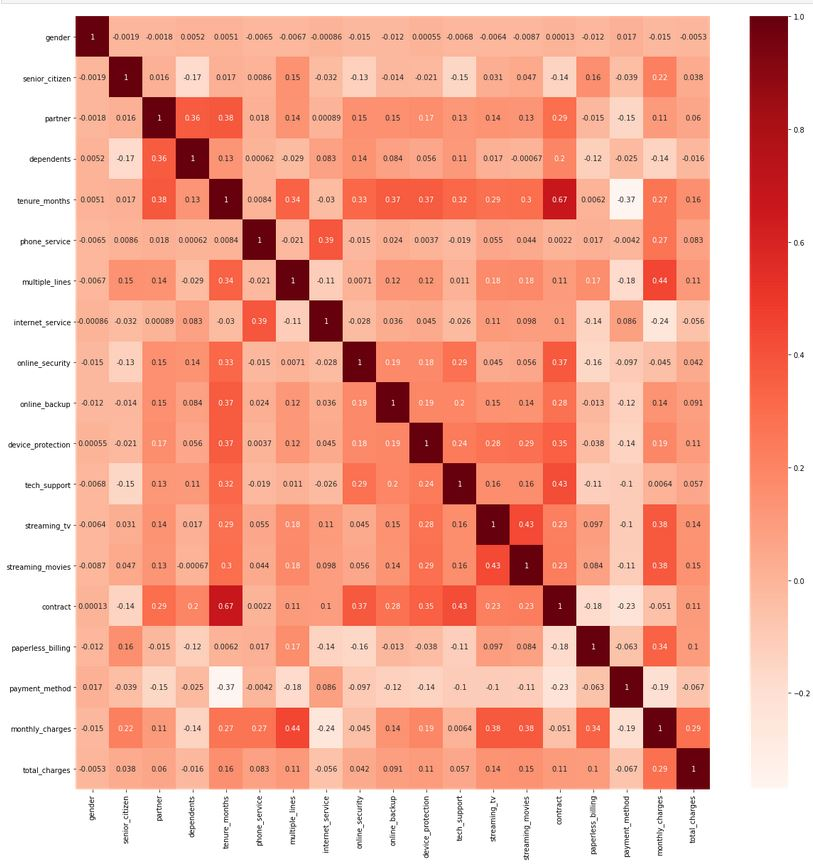
\includegraphics[scale=0.5]{photos/heatmap.JPG}
\end{figure}

\begin{figure}
    \centering
    \begin{minipage}{0.45\textwidth}
        \centering
        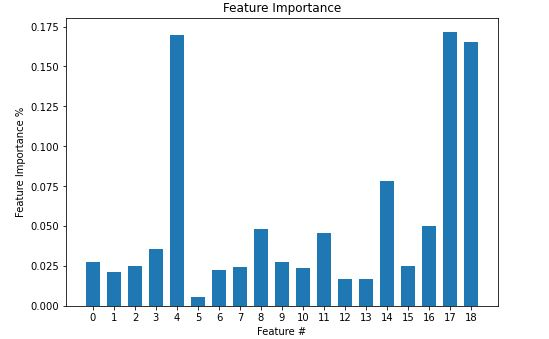
\includegraphics[width=0.9\textwidth]{photos/feautreImportanceBeforeDrop.JPG}
        \caption{Feature Importance With All Features}
    \end{minipage}\hfill
    \begin{minipage}{0.45\textwidth}
        \centering
        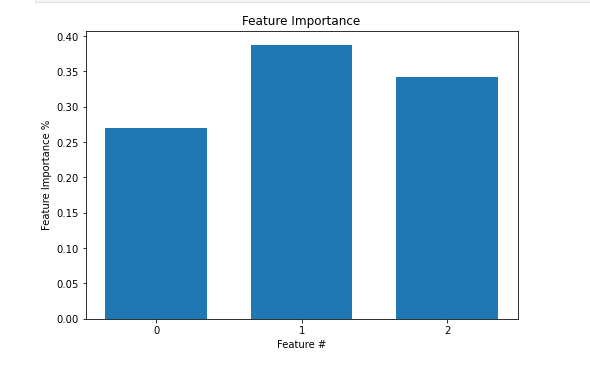
\includegraphics[width=0.9\textwidth]{photos/feauresAfterDrop.png}
        \caption{Feature Importance After Dropping Features}
    \end{minipage}
\end{figure}
\subsection{Model Building}

To build the first model we will take all of the available 18 features and pass them into a Random Forest Classifier model to get a baseline of how accurate the model can be using all of the features. In the case of using the 18 features the model is able to achieve 79.8\% accuracy. We can see in Figure 2 that there are relatively few features that suggested to provide a lot of importance to the model, these features included: tenure\_months, monthly\_charges, total\_charges.

By dropping the other features and only keeping the 3 highly contributing features, the second model was able to achieve 75\% accuracy, although the model is losing nearly 5\% of the accuracy.

Using the suggested 10 features from step backward feature selection the model is able to achieve 77.8\% accuracy. Reducing the overall number of features from 18 but still having a little over 3 times as many features as the previous model.



\subsection{Model Evaluation}
As we can observe from the results, the model with all of the features is producing the best results. The downside to this model is that we are having to use all of the features which in this case is not a problem since the number of features is relatively small and does not require a lot of processing time.

However, the model with 3 features is able to achieve similar levels of accuracy as the model with all 18 features despite having a \( \frac{1}{6} \) of the features. Although the model does take a hit in accuracy, as it loses nearly 5\% of the accuracy that the model with 18 features has, the reduction in features is significant.

In the model that used the features from step backward feature selection, the results are middling. The number of features are reduced to 10 from 18, and achieves slightly worse accuracy compared to the 18 features model but slightly better accuracy than the 3 features model.
\section{Results \& Discussion}
Predicting churn and finding informative characteristics of customer churn is definitely achievable. The models using Random Forest Classifier were all able to achieve relatively good results with varying amounts of features. The filter method used in this paper was not able to help reduce the overall number of features but using the feature\_importance attribute provided by Random Forest Classifier we were able to find which features would be highly valued in the model, allowing us to reduce the overall number of features. Step backward and step forward feature selection were also able to provide valuable insight that there was definitely room to reduce the features while maintaining higher levels of accuracy.
\begin{figure}
    \centering
    \begin{minipage}{0.45\textwidth}
        \centering
        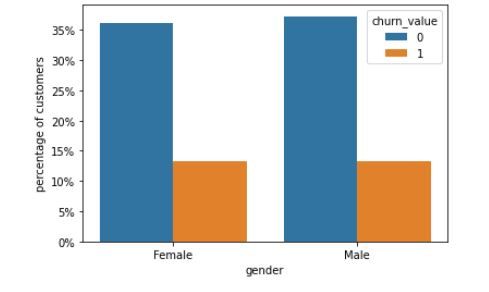
\includegraphics[width=0.9\textwidth]{photos/genderChurnBarChart.JPG}
        \caption{Churn by Gender}
    \end{minipage}\hfill
    \begin{minipage}{0.45\textwidth}
        \centering
        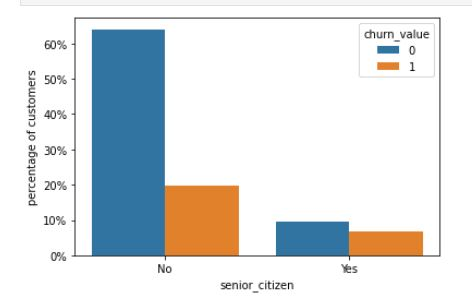
\includegraphics[width=0.9\textwidth]{photos/seniorCitizenVsNonSeniorCitizenBarChart.JPG}
        \caption{Senior Citizen Churn vs Non-Senior Citizen Churn}
    \end{minipage}
\end{figure}

We can also observe that the data set shows that there is no discernible difference between churners by gender, both men and women seem to churn at nearly the same rate. The interesting piece in this data, is that it is suggested that even though senior's makeup a small part of the overall data, they happen to be contributing at nearly double the rate that non-senior citizens churn. Possibilities for this phenomenon could be related to declining health of senior citizens, or no longer being able to afford payments. There does seem to be a research gap in understanding the reason for this unusually high churn rate among senior citizens.

\section{Conclusion}
With the amount of competition between companies, it is important for businesses to tap every potential source of revenue. Churn prediction is important for modern companies, and not just in financial sectors. Churn prediction can be applied to other sectors, such as reducing churn with students or looking into employee retention. Understanding why people are leaving is ultimately the goal shared between all sectors involved with reducing churn. Pinpointing why customers are leaving will allow companies to reduce churn, and predict potential churners to further increase retention and save costs that would otherwise go to expensive customer acquisition campaigns. Modern machine learning has made predicting potential churners and finding the causes much easier than it would have been in the past, companies can identify the customers that require extra attention and apply various strategies based on that customers habits to try and retain them. Although hiring data scientists may in itself be expensive, the benefits of having an understanding of your customer base is invaluable.\\
\bibliographystyle{plain}
\bibliography{references}

\end{document}